\section{Object definitions and Event selection}

\subsection{Event cleanup and vertex selection}

Events with at least one primary vertex passing an OR combination
of the HLTs shown on table \ref{tab:HLTDatasets}, and containing at least three
preselected leptons (number of muons plus number of electrons) are selected
provided that its missing energy $E_T^{Miss}$ is greater than $40~GeV$.

In addition, the following flags are required for the event:

\begin{itemize}
  \item \verb|Flag_goodVertices|
  \item \verb|Flag_globalSuperTightHalo2016Filter|
  \item \verb|Flag_HBHENoiseFilter|
  \item \verb|Flag_HBHENoiseIsoFilter|
  \item \verb|Flag_EcalDeadCellTriggerPrimitiveFilter|
  \item \verb|Flag_BadPFMuonFilter|
\end{itemize}

One additional flag is required for the year 2017, 2018:

\begin{itemize}
\item \verb|Flag_ecalBadCalibFilterV2|
\end{itemize}

Events are then splitted in four channels depending on the leptonic flavour of the
diboson decay:

\begin{description}
\item[$\bullet$3e] three electrons and missing transverse energy are found, two of the
  electrons correspond to the decay of the $Z$ boson and the remaining electron corresponds
  to the decay of the $W$ boson. $Z\rightarrow e^{+}e^{-} W\rightarrow e+\nu$
  The three electrons are expected to leave traces on the
  tracker subsystem with low curvature due to their high transverse momentum and
  energy depositions are expected in the electromagnetic calorimeter
  The signature left on the CMS detector is shown on figure \ref{fig:Fireworks_eeev}.
\item[$\bullet$2e+1mu] two electrons, one muon and missing transverse energy are found,
  the two electrons correspond to the decay of the $Z$ boson and the muon corresponds to the
  decay of the $W$ boson. $Z\rightarrow e^{+}e^{-} W\rightarrow \mu+\nu$ the two electrons are
  expected to leave traces on the tracker subsystem with low curvature and energy
  depositions are expected in the electromagnetic calorimeter while the muon leaves
  traces in the tracker and muon subsytem. The signature left on the CMS
  detector is shown on figure \ref{fig:Fireworks_eemuv}.
\item[$\bullet$2mu+1e] two muons, one electron and missing transverse energy are found,
  the two muons correspond to the decay of the $Z$ boson and the electron corresponds to the
  decay of the $W$ boson. $Z\rightarrow \mu^{+}\mu^{-} W\rightarrow e+\nu$ the two
  muons leave traces on the tracker and muon subsystems with negligible curvature due
  to its high transverse momentum while the electron is expected to leave hits in
  the tracker and energy deposition in the electromagnetica calorimeter.
  The signature left on the CMS detector is shown on figure \ref{fig:Fireworks_mumuev}.
\item[$\bullet$3mu] three muons and missing transverse energy are found, the muon pair
  correspond to the decay of the $Z$ boson and the remianing muon corresponds
  to the decay of the $W$ boson. $Z\rightarrow \mu^{+}\mu^{-} W\rightarrow \mu+\nu$.
  The three muons are expected to leave traces on the tracker subsystem and muon chambers
  with low curvature due to their high transverse momenta. The signature
  left on the CMS detector is shown on figure \ref{fig:Fireworks_eemuv}.
\end{description}

\begin{figure}
  \centering
  \subfigure[Projection on the $\rho-\phi$ plane. \label{fig:A_RhoPhi}]{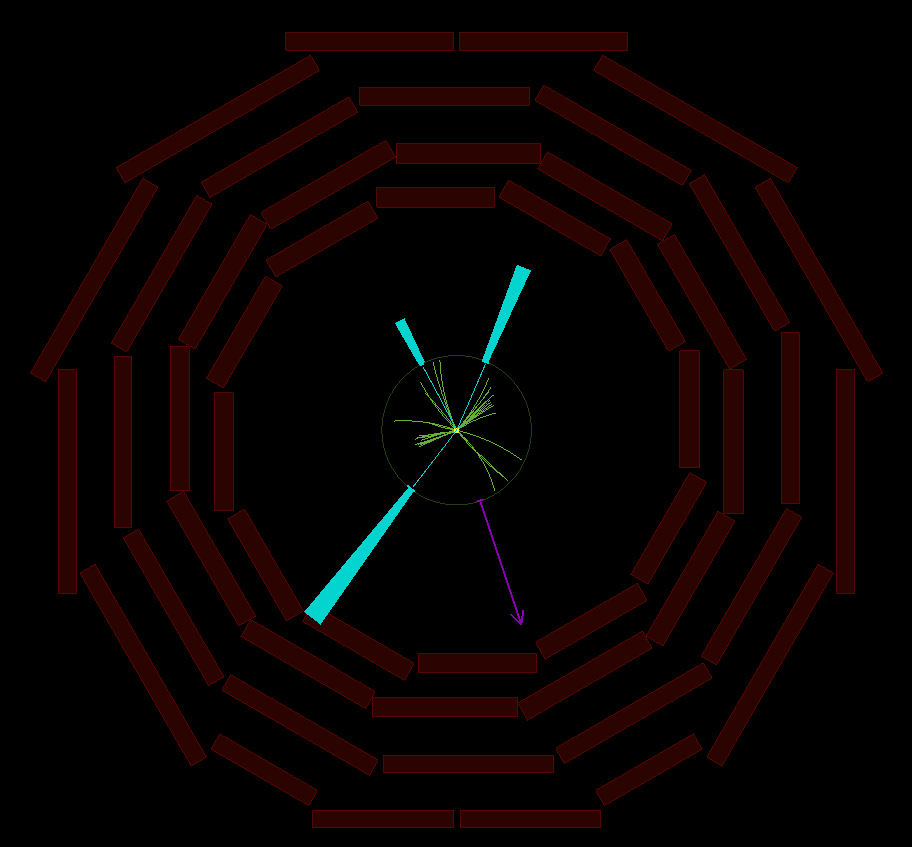
\includegraphics[width=0.8\linewidth]{fig/Fireworks/A_RhoPhi.png}}
  \vfil
  \subfigure[Projection on the $\rho-z$ plane\label{fig:A_RhoZ}]{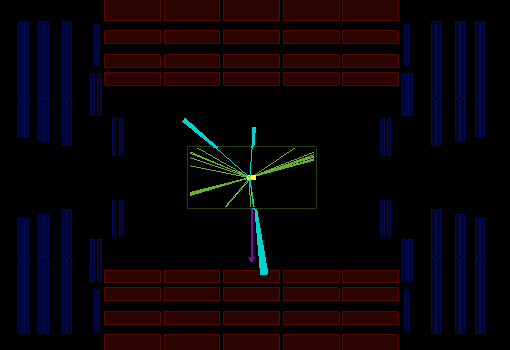
\includegraphics[width=0.40\linewidth]{fig/Fireworks/A_RhoZ.png}}
  \subfigure[3D view\label{fig:A_Rho3D}]{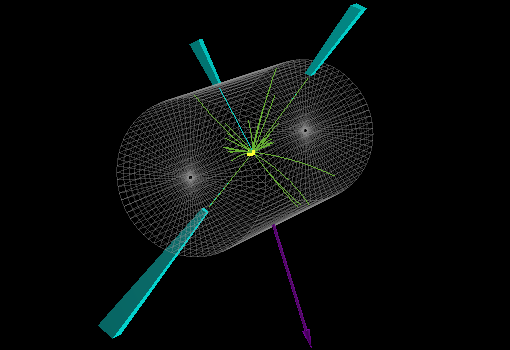
\includegraphics[width=0.40\linewidth]{fig/Fireworks/A_3D.png}}
  \caption{Example of the signature left on the detector by a signal-like event
    for the $eee\nu$ channel. This event was taken on July 13th 2018. Run: $319579$,
    Lumiblock: $2957$, Event: $4487890911$. The reconstructed primary vertex is shown in yellow.
    Depositions on the electromagnetic calorimeter and tracks left by the three electrons
    are shown in turquoise, the negligible curvature
    shown by their tracks is a reflection of their high transverse momentum.
    The amount of missing transverse energy is proportional to the length of the purple arrow. Low momentum
    tracks for particle-flow candidates in the inner tracker are shown in green for
    reference, these PF candidates are filtered by the preselection. }
  \label{fig:Fireworks_eeev}
\end{figure}


\begin{figure}
  \centering
  \subfigure[Projection on the $\rho-\phi$ plane. \label{fig:B_RhoPhi}]{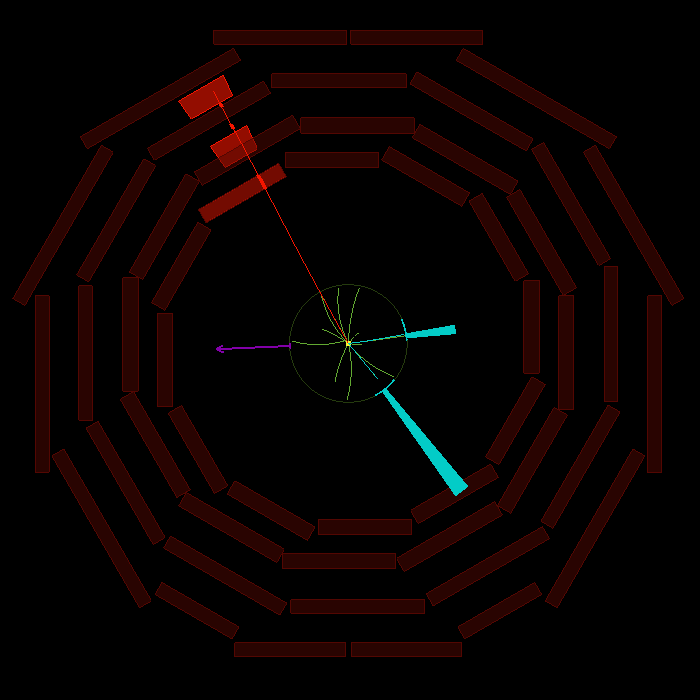
\includegraphics[width=0.8\linewidth]{fig/Fireworks/B_RhoPhi.png}}
  \vfil
  \subfigure[Projection on the $\rho-z$ plane\label{fig:B_RhoZ}]{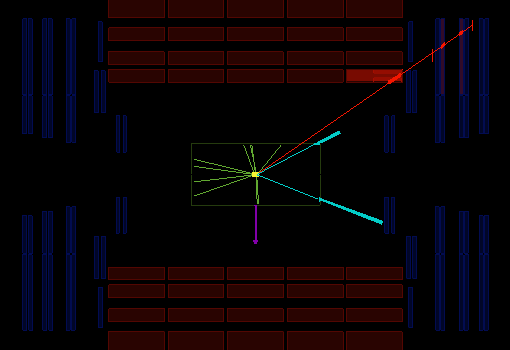
\includegraphics[width=0.40\linewidth]{fig/Fireworks/B_RhoZ.png}}
  \subfigure[3D view\label{fig:B_Rho3D}]{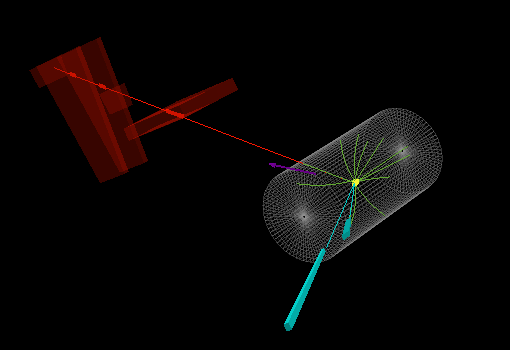
\includegraphics[width=0.40\linewidth]{fig/Fireworks/B_3D.png}}
  \caption{Example of the signature left on the detector by a signal-like event
    for the $ee\mu\nu$ channel. This event was taken on October 21st 2018. Run: $32500$,
    Lumiblock: $188$, Event: $346288517$. The reconstructed primary vertex is shown in yellow.
    Depositions on the electromagnetic calorimeter
    and tracks left by the electronic pair are shown in turquoise, the negligible curvature
    shown by their tracks is a reflection of their high transverse momentum. Tracks left by the muon
    in the tracker detector and muon chambers are shown in red, in this particular event it
    is possible to see the muon will be classified as a global-High Pt muon as its traces
    are found in the tracker system and beyond the first station of the muon subsystem.
    The amount of missing
    transverse energy is proportional to the length of the purple arrow. Low momentum
    tracks for particle-flow candidates in the inner tracker are shown in green for
    reference, these PF candidates are filtered by the preselection. }
  \label{fig:Fireworks_eemuv}
\end{figure}

\begin{figure}
  \centering
  \subfigure[Projection on the $\rho-\phi$ plane. \label{fig:C_RhoPhi}]{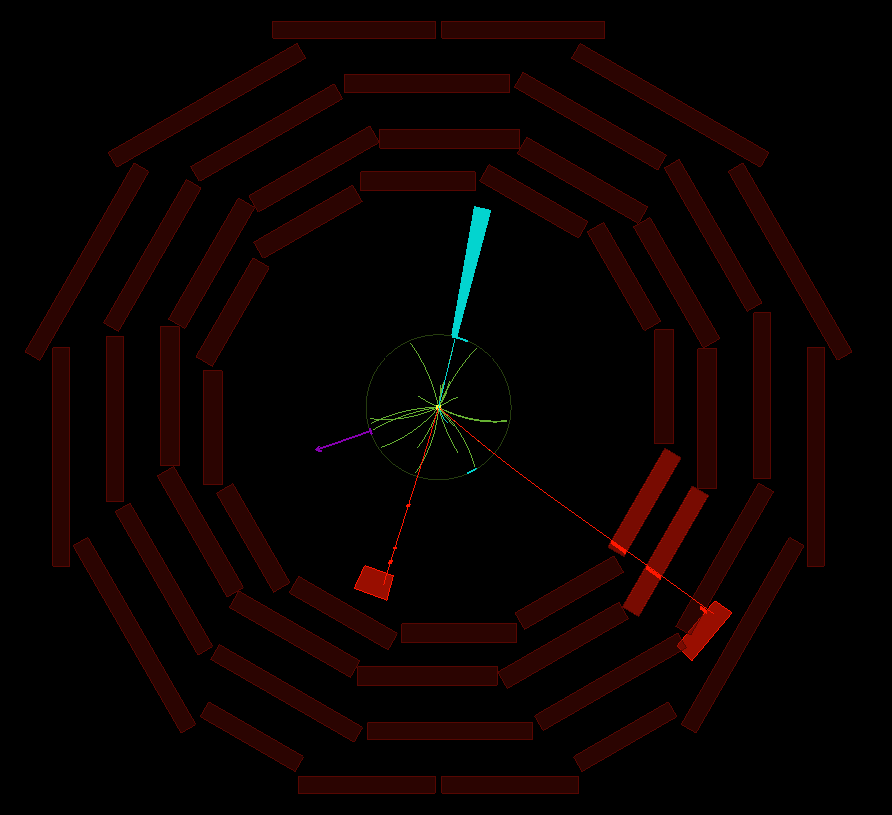
\includegraphics[width=0.8\linewidth]{fig/Fireworks/Cv2_RhoPhi.png}}
  \vfil
  \subfigure[Projection on the $\rho-z$ plane\label{fig:C_RhoZ}]{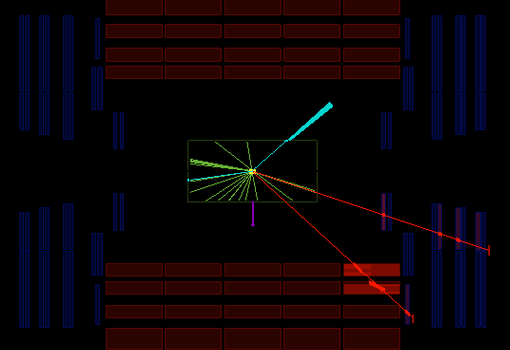
\includegraphics[width=0.40\linewidth]{fig/Fireworks/Cv2_RhoZ.png}}
  \subfigure[3D view\label{fig:C_Rho3D}]{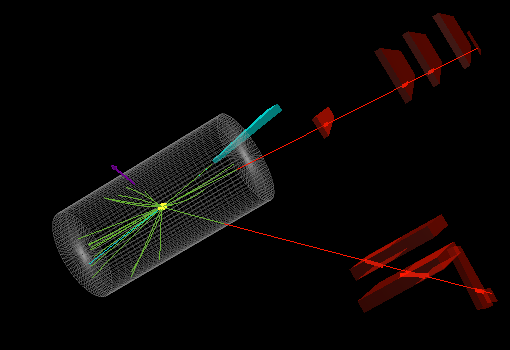
\includegraphics[width=0.40\linewidth]{fig/Fireworks/Cv2_3D.png}}
  \caption{Example of the signature left on the detector by a signal-like event
    for the $\mu\mu e \nu$ channel. This event was taken on October 1st 2018.
    Run: $323790$, Lumiblock: $376$, Event: $646065569$. The reconstructed primary vertex is shown in yellow.
    The deposition on the electromagnetic calorimeter and tracks left by the electron are shown in turquoise,
    the negligible curvature shown by their tracks is a reflection of their high transverse momentum.
    Tracks left by the muon pair in the tracker detector and muon chambers are shown in red. It
    is possible to see one of the muons will be classified as a tracker-High Pt muon as its traces
    are found in the tracker system and the first muon station while the other one is a global-High Pt
    Muon as its muon trackes go beyond the first station of the muon subsystem.
    The amount of missing
    transverse energy is proportional to the length of the purple arrow. Low momentum
    tracks for particle-flow candidates in the inner tracker are shown in green for
    reference, these PF candidates are filtered by the preselection. }
  \label{fig:Fireworks_mumuev}
\end{figure}

\begin{figure}
  \centering
  \subfigure[Projection on the $\rho-\phi$ plane. \label{fig:D_RhoPhi}]{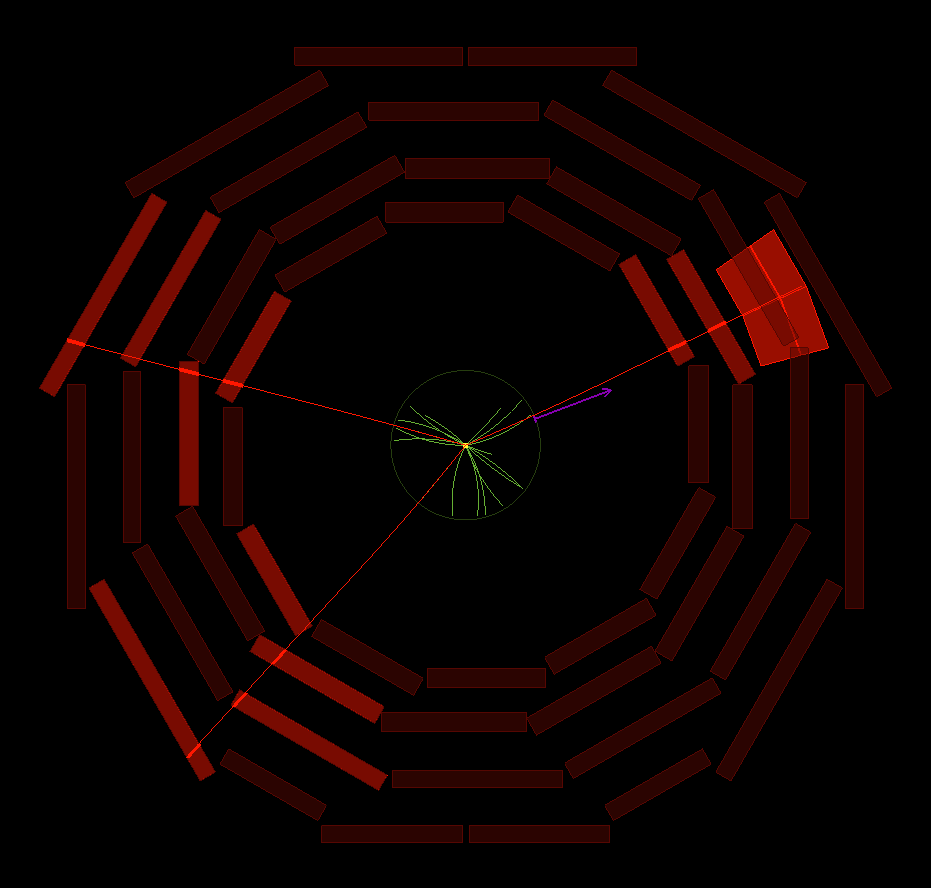
\includegraphics[width=0.8\linewidth]{fig/Fireworks/D_RhoPhi.png}}
  \vfil
  \subfigure[Projection on the $\rho-z$ plane\label{fig:D_RhoZ}]{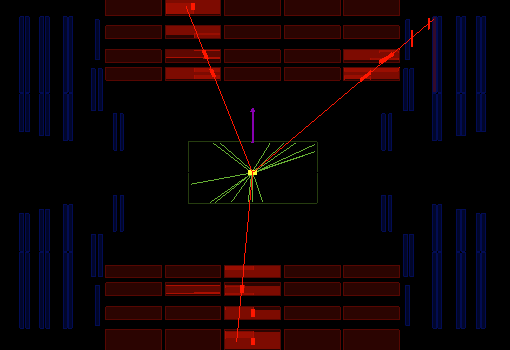
\includegraphics[width=0.40\linewidth]{fig/Fireworks/D_RhoZ.png}}
  \subfigure[3D view\label{fig:D_Rho3D}]{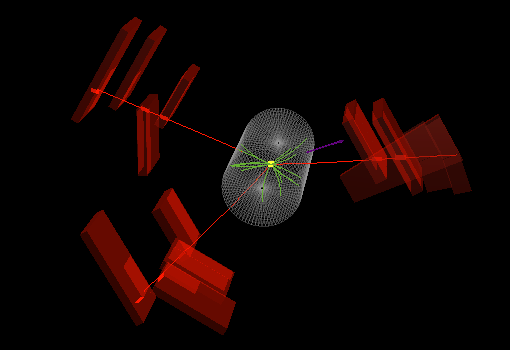
\includegraphics[width=0.40\linewidth]{fig/Fireworks/D_3D.png}}
  \caption{Example of the signature left on the detector by a signal-like event
    for the $\mu\mu\mu\nu$ channel. This event was taken on July 21st 2018.
    Run: $320024$, Lumiblock: $211$, Event: $355149645$. The reconstructed primary vertex is shown in yellow.
    Tracks left by the muon pair in the tracker detector and muon chambers are shown in red,
    the negligible curvature shown by their tracks is a reflection of their high transverse momentum.
    it is possible to see the muon will be classified as a global-High Pt muon as their traces
    are found in the tracker system and beyond the first station of the muon subsystem.
    The amount of missing
    transverse energy is proportional to the length of the purple arrow. Low momentum
    tracks for particle-flow candidates in the inner tracker are shown in green for
    reference, these PF candidates are filtered by the preselection. }
  \label{fig:Fireworks_mumumuv}
\end{figure}






\subsection{High Level Trigger Selection}

Table \ref{tab:HLTDatasets} shows the HLTs and the different datasets used for the three years.
Due to the presence of multiple leptonic flavors in the final state, each event
is required to pass either the Muon or Electron triggers based on the high-Pt
recommendations from the POG.


\subsection{Lepton Selection}

\subsection{Electron Selection}

\verb|Electron| collection in \verb|NanoAOD|

Electrons are reconstructed from hits in the different
layers of the tracker and energy deposits in the scintillating crystalls
across the $\eta-\phi$ plane in the Electromagnetic Calorimeter.

The electron's sign charge can be identified by its signature in the tracker
due to the presence of the strong magnetic field in the CMS detector.

Electrons in this analysis are required to be within the ECAL fiducial
region i.e $\abs{eta}<2.5$ excluding the transition region betwen the
barrel and the endcaps $1.4442<\abs{eta}<1.5660$.

\begin{figure}[tph]
  \centering
  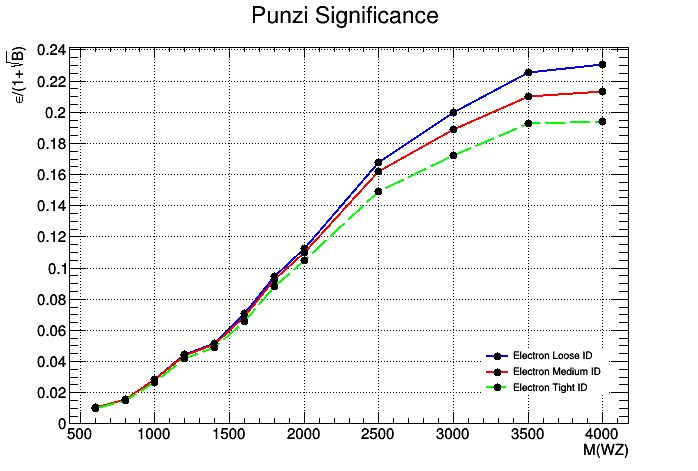
\includegraphics[width=0.6\textwidth]{fig/LeptonIDStudies/ElectronIDPunzi.png}
  \caption{Punzi significance for the different Electron's cut-based IDs for the
    electron decay $Z\rightarrow e+e$. The cut-based loose ID shows high efficiency
    specially at high masses where the distance in the $\eta-\phi$ plane is
    expected to be small.}
  \label{fig:PunziElectronIDs}
\end{figure}

Electron identification is based on a cut based ID as defined by the
EGamma POG. Depending on the channel, this requirement
may ask for \emph{loose} or \emph{tight} electrons, the former with an
average efficiency of approximately 95\% and 70\% for
the latter ~\cite{EGammaPOG_el}: channels portraying a $Z\rightarrow e+e$
decay ($eee\nu$ and $ee\mu\nu$) require two loose
electrons due to its high efficiency, specially at high resonant mass where
the electrons are expected to be highly collimated (see Figure \ref{fig:PunziElectronIDs}).
The electron corresponding to the $W\rightarrow e\nu$ decay is required to pass
the cut-based tight ID.

We reproduce the High Level Trigger transverse momentum requirements by
applying a cut on the corresponding $p_T$ threshold on all
preselected electrons:
2016 ($27~GeV$), 2017 ($35~GeV$), and 28 ($32~GeV$).

\subsection{Muon Selection}

\verb|Muon| collection in \verb|NanoAOD|

The muon objects in this analysis can be divided into two categories:
Tracker and Global highPt muons ~\cite{MuonPOG}. Tracker highPt muons are
reconstructed from hits in the tracker matched with hits in the first
muon station, while global highPt muons leave trace beyond the first
layer of the muon subsystem.

Muons are required to be within the pseudorapidity range $\abs{eta}<2.4$ and
to have a minimum transverse momentum of $P_t=20$. Additionally the leading muon
is required to have a transverse momentum $P_t>52~GeV$ in line with
the trigger plateau.



\begin{figure}[tph]
  \centering
  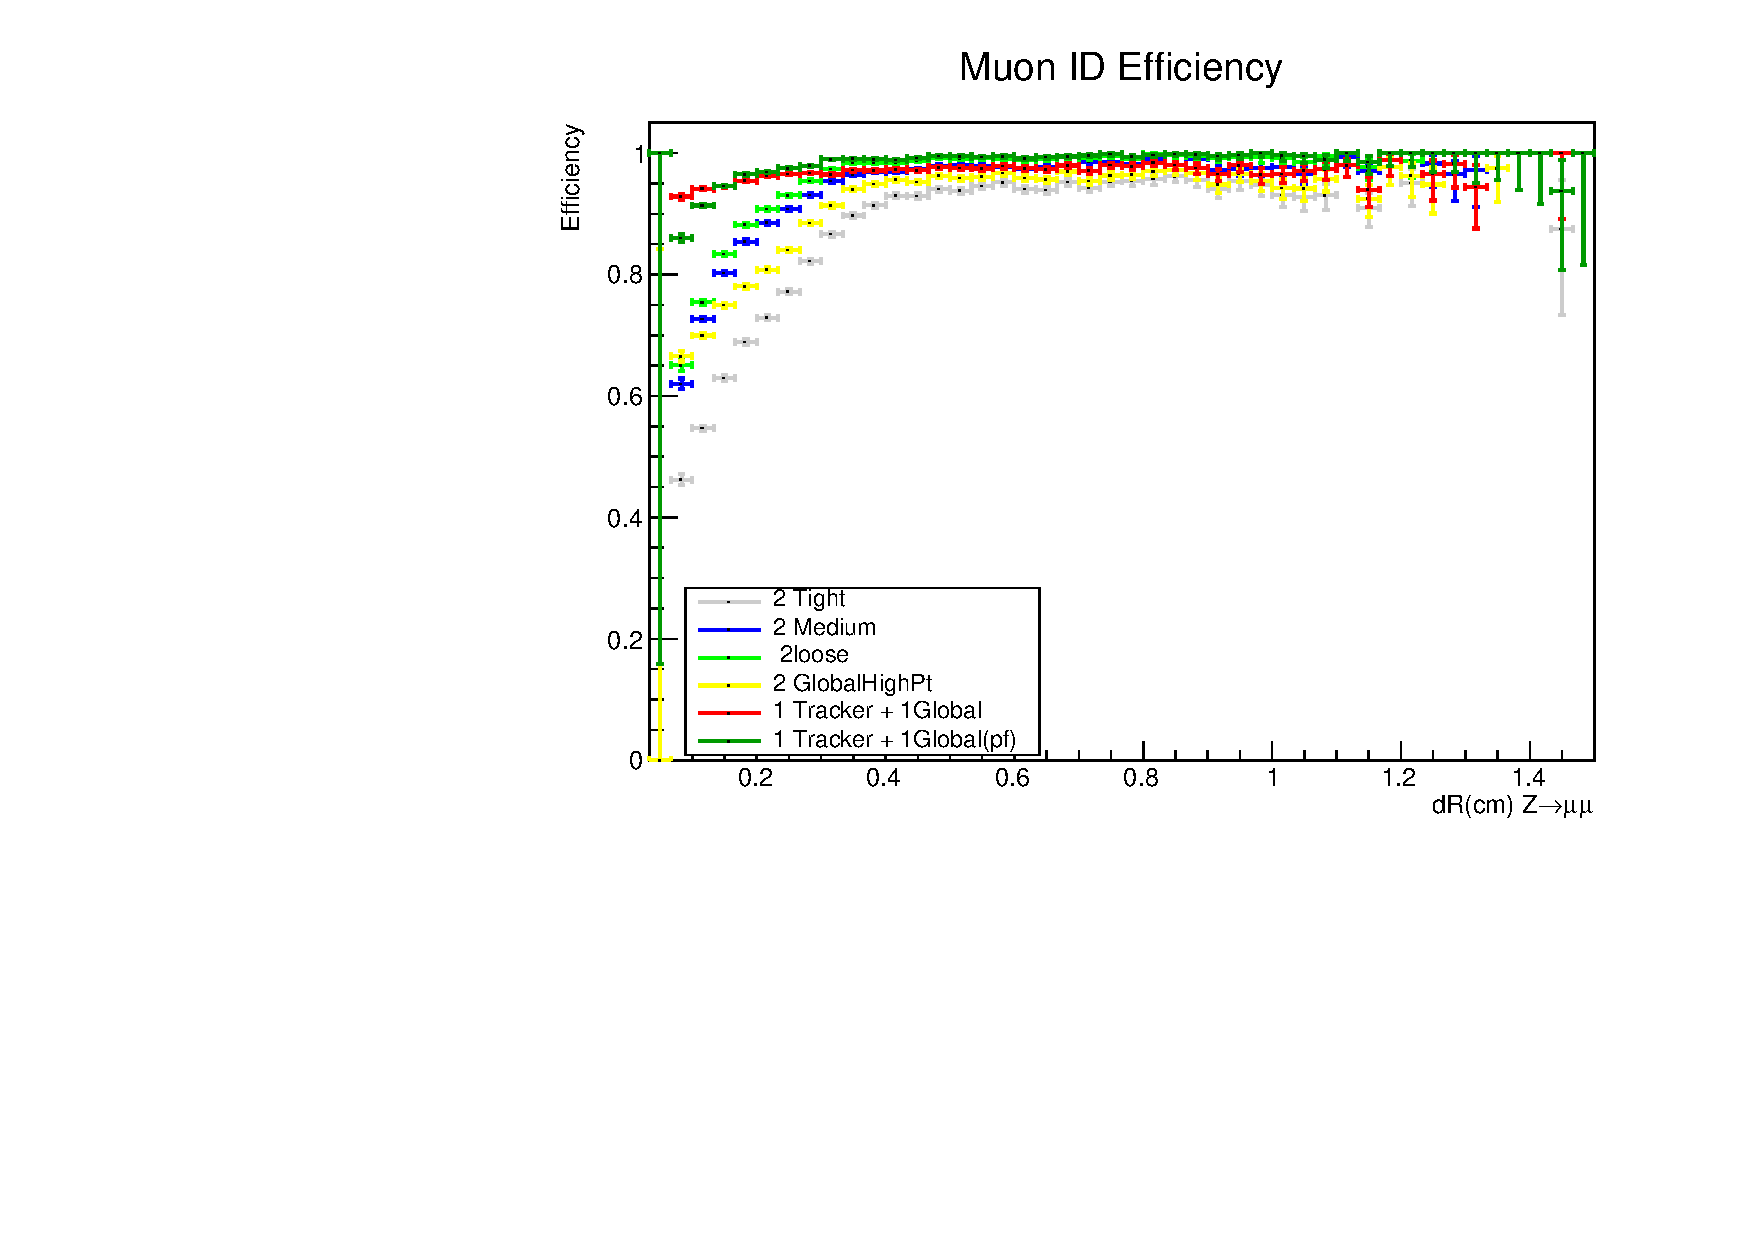
\includegraphics[width=0.6\textwidth]{fig/LeptonIDStudies/MuonIDEfficiency.pdf}
  \caption{Signal Efficiency for different Muon ID combinations for the product of
    the decay $Z\rightarrow\mu+\mu$. The less efficient combination is requiring
    the Muon pair to be a cut-based Tight ID pair, increasing efficiency towards less
    strict cut-based requirements (Loose and Medium ID). The most efficient combination in
    the signal reconstruction is the combination of one global-highPt ID Muon
    with another muon that can be either a tracker or global-HighPt ID.}
  \label{fig:MuonIDEfficiency}
\end{figure}

For events portraying a $Z\rightarrow\mu+\mu$ decay a stricter cut is applied on the
leading muon $P_{t}>70~GeV$. The muon pair is required to be a composite of a
cut-based global highPt ID muon and either a tracker or global highPt ID muon
that is simultaneously a particle-flow candidate. This combination of highPt
muons shows the highest efficiency, see Figure \ref{fig:MuonIDEfficiency}.
%%% Add reference to B2G-19-006 %%%

Events with a pair of muons with an impact parameter $ip3d>0.01~cm$ are
discarded in order to increase background rejection.

\subsection{Lepton Misidentification}


\begin{figure}[tph]
  \centering
  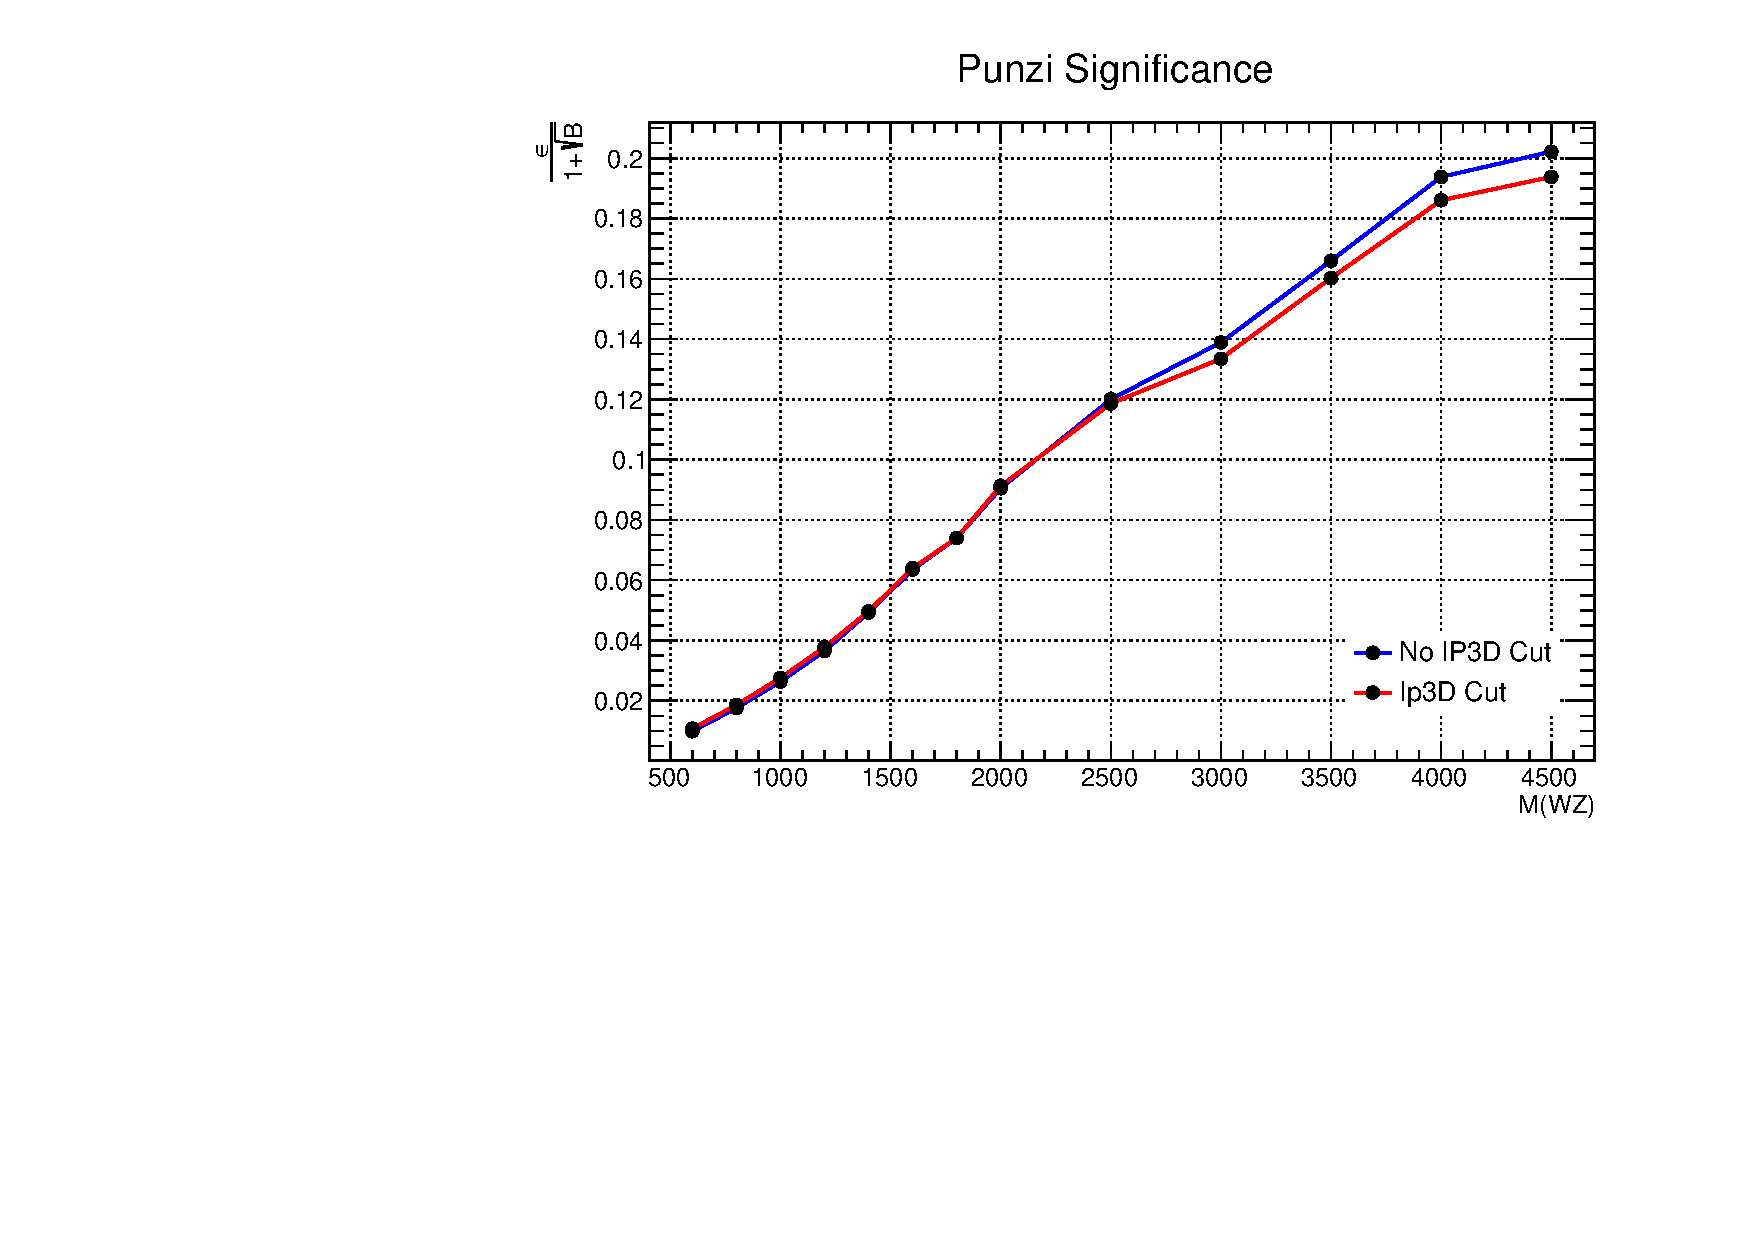
\includegraphics[width=0.6\textwidth]{fig/PunziTest_Ip3DCut.pdf}
  \caption{Punzi significance as a function of the mass resonce prior to and after implementing
    the cut on the impact parameter in order to reduce the number of non-prompt
    muons}
  \label{fig:Punzi_Ip3DCut}
\end{figure}

The nature of the reconstruction process may lead to some objects being
wrongly identified. A dedicated study was performed in order to evaluate
the effects on misreconstructed objects on the counting experiment.
Misreconstructed leptons are also commonly refered as fake leptons. It
is assumed that if the number of MC generated electrons (muons) match
the number of reconstructed electrons (muons) there are no misreconstructed
objects. A fake lepton is a lepton that is non-prompt that didn't arise from
a $\tau$ lepton or from a heavy flavour decay (HFD). Figure %%Missing Figure %%%
shows how the Drell-Yan and $t\bar{t}$ processes are suceptible to present
reconstructed non-prompt muons. To account for this, we impose a cut on the
3D impact parameter $ip3D<0.01~cm$, figure %%Missing Figure %%%
shows the effect of the cut on reducing the number of non-prompt muons.
The Punzi significance of the impact parameter requirement as a function
of the WZ resonance mass is shown in figure \ref{fig:Punzi_Ip3DCut}. %%% expand %%%


\begin{figure}[tph]
  \centering
  \subfigure[Lepton origin classification prior to constraining the impact parameter]
            {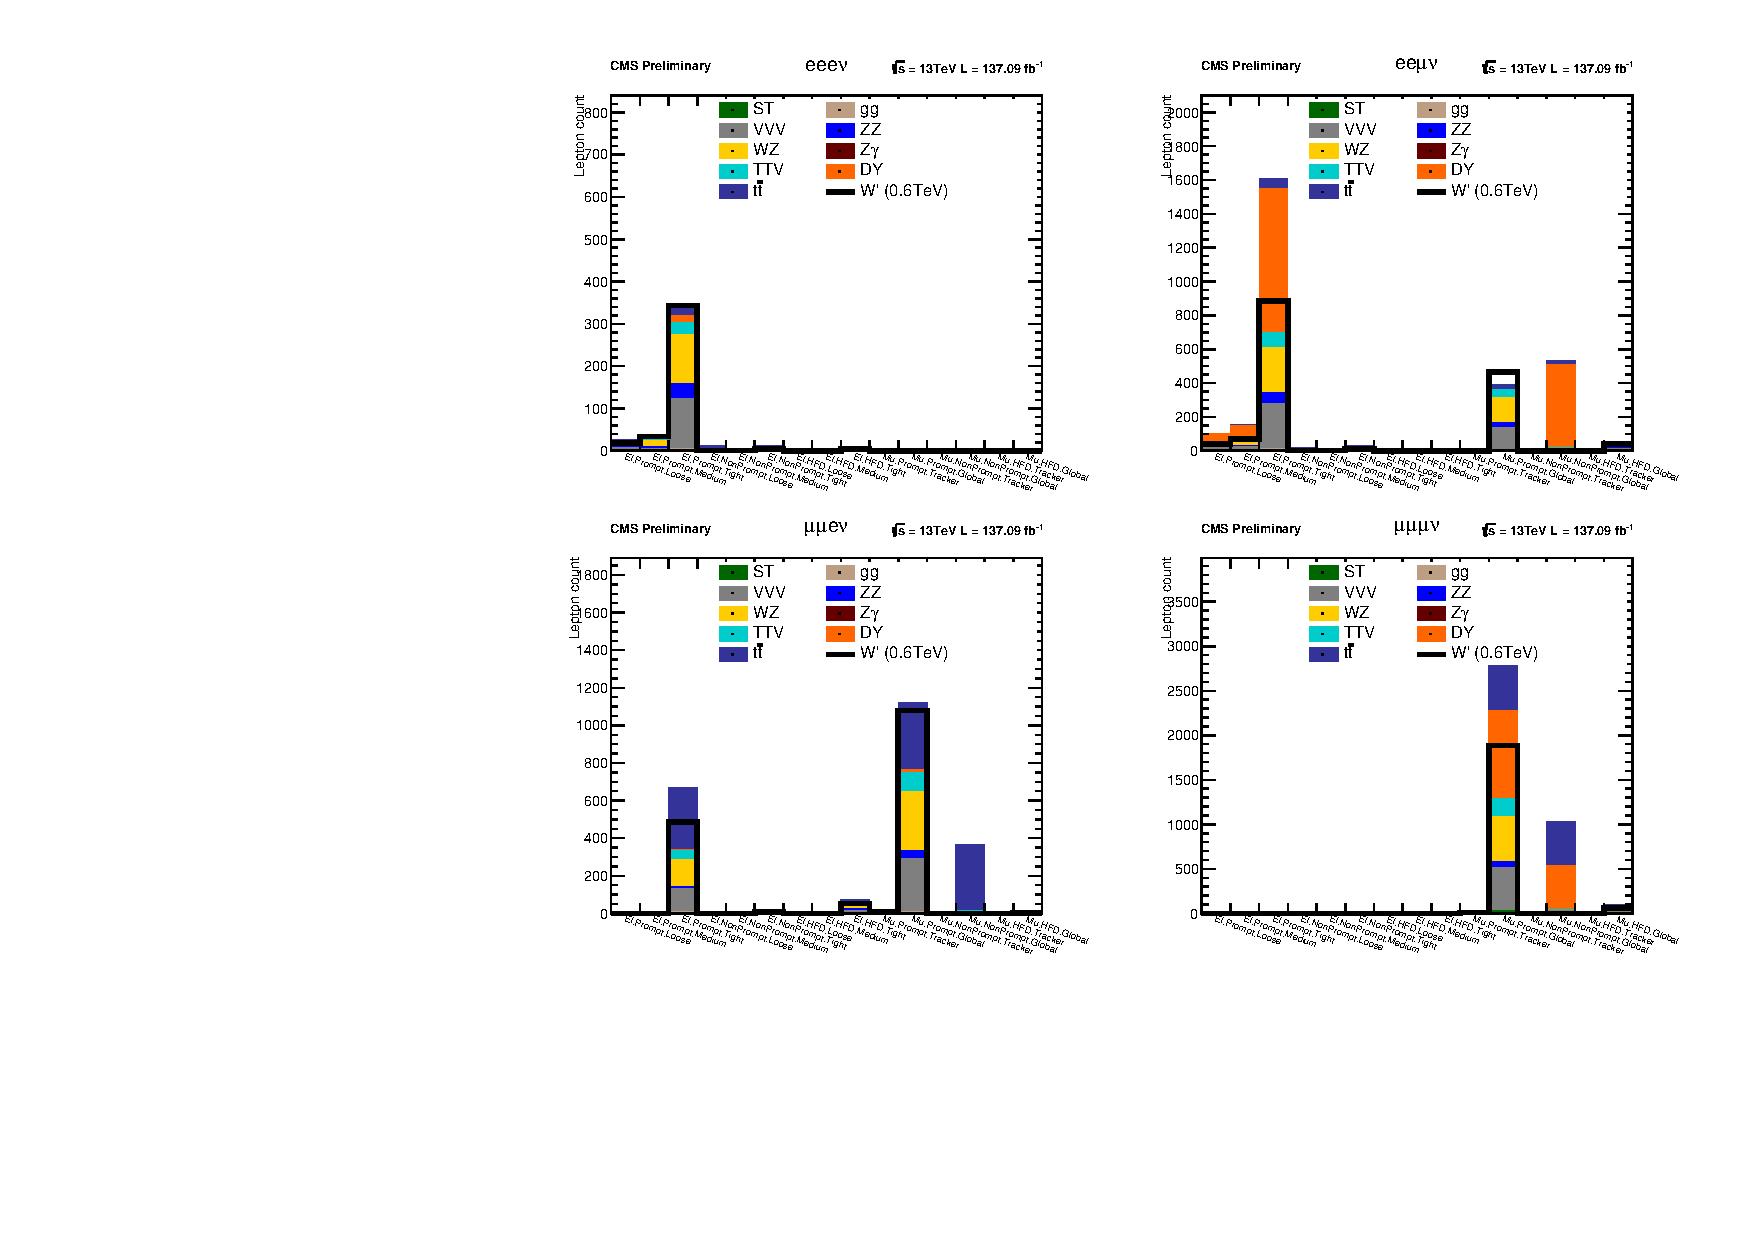
\includegraphics[width=.8\textwidth]{fig/Run2/NoIp3DCut_HFakeString_SR1_A_RuRun2_M600.pdf}}
  \vfil
  \subfigure[Lepton origin classification after constraining the impact parameter $ip3D<0.01~cm$]
            {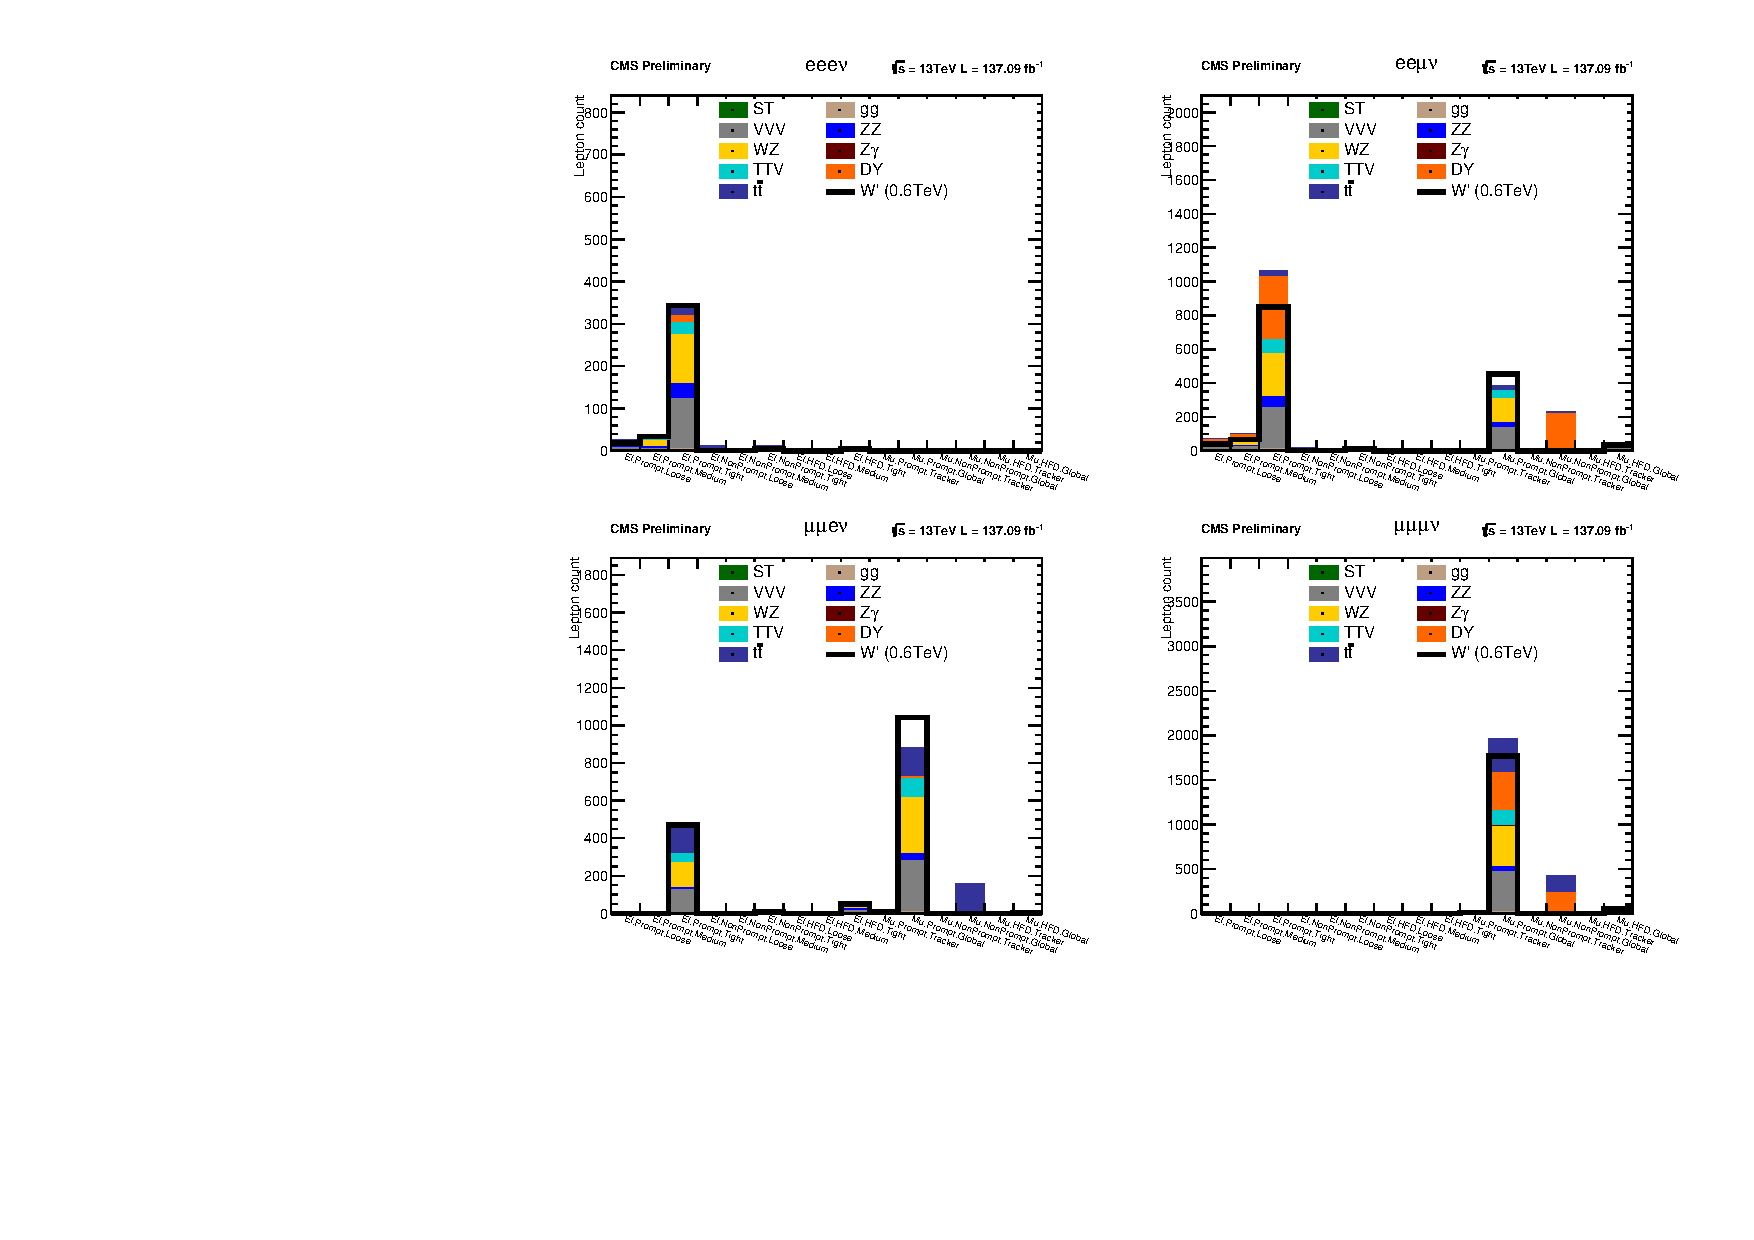
\includegraphics[width=.8\textwidth]{fig/Run2/Rebining_HFakeString_SR1_A_RuRun2_M600.pdf}}
  \caption{Lepton origin classification according to simulation prior and after applying
    an impact parameter requirement $ip3D<0.01~cm$. Each lepton is considered individually
    when filling the histogram. The main contribution to non-prompt leptons come
    from Muons in Drell-Yan and $t\bar{t}$ events.
  }
  \label{fig:HFakeString}
\end{figure}


\subsection{Missing Transverse Energy}

The missing transverse energy $E_T$ is reconstructed with the particle flow
algorithm ~\cite{particleflow} and events are required to have at least a
missing transverse energy of $E_T^{miss}=40~GeV$.

\subsection{Z Candidate}

Two same flavored, opposite charged leptons are required to reconstruct a Z
candidate. If more than one pair is found, the one with reconstructed mass
closer to the nominal mass $M_z=91.1876~GeV$ is chosen. The pair's mass
is required to fall in the Z mass window $70~GeV < M_Z < 111~GeV$. In favor of an
increase in the signal efficiency the opposite charged requirement is dropped
for the $eee\nu$ category.

If the Z candidate is formed from a muon pair with a leading (subleading) muon with
a transverse momentum of at least $P_t=70 GeV$ ($P_t=10GeV$). One of the
muons is required to pass two additional requirements: being a global high-Pt muon and a
particle-flow candidate. In the case of electrons, the requirement is to pass the
selection criteria of the cut-based \emph{loose} ID and a transverse momentum of
matching the trigger plateau.

The event is rejected from the signal region if the distance in the $\eta-\phi$
plane for the two leptons product of the decay of the Z is less than $1.5$.

\subsection{W Candidate}

The $W$ candidate is reconstructed from the remaining lepton and the missing energy
of the event $E_T^{miss}$. The ramining lepton is required to be either a cut based \emph{tight}
ID electron or a global High-Pt muon with a transverse momentum
of at least $Pt>52~GeV$.

The neutrino from the $W \rightarrow l\nu$ decay escapes undetected,
and therefore the following assumptions are made in order to perform a kinematic
reconstruction of the $W$ candidate: there are no additional sources of missing
energy, and consequently $E_{Pt}^{miss}$ is considered the transverse momentum
corresponding to the undetected neutrino. The longitudinal momentum $P_z$ can be
recovered by imposing the $M_W=80.379~GeV $ nominal mass and assuming
a massless neutrino $M_\nu = 0.$

As $\eta$ is unknown for the missing transverse energy, the neutrino 4-vector is
not well defined. However, by assuming the mass of $W$ the longitudinal component
of the neutrino is reduced to a quadratic equation:

\[
P_{Z}^{\nu} = \frac{P_{Z}^{l}({M_{W}^{2}-{M_{t}^{W}}^2+2P_{t}^{l}{P_{t}^{\nu}}}) \pm P^{l}\sqrt{(M_{W}^{2}-{M_{t}^{W}}^2)((M_{W}^{2}-{M_{t}^{W}}^2)+4P_{t}^{l}P_{t}^{\nu})}}{{2P_{t}^{l}}^{2}}
\]

Where the transverse mass $M_{t}^{W}$ is defined
as ${M_{t}^{W}}=\sqrt{2P_{t}^{l}P_{t}^{\nu}(1-cos\phi_{l\nu})}$.
Due to detector resolution effects and systematic uncertainties on the
reconstruction of missing transverse energy, the transverse mass may
exceed the mass of the $W$ boson $M_W$ and the
longitudinal component of the momentum would remain undefined, in these cases
we set the transverse mass equal to the nominal value $M_{t}^{W}=M_W$.

The less energetic of the solutions gives the correct value ~70\% of the time
according to simulation [AN].
When no real solutions are available (transverse mass > W Mass), the invariant
mass is set to the reconstructed transverse mass and we are left with two real
identical solutions.


\subsection{WZ Candidate}

The $W^{\prime}$ is reconstructed from the $W$ and $Z$ candidates.
Events are rejected if the sum of the leptonic mass is less than $120~GeV$ and
if the sum of the transverse momentum $L_{t}<110~GeV$, where $L_{t}$ is defined
as:

\[
L_{t} = \sum_{n=1}^{3} Pt_{ln}
\]






